% Slides for lab retreat
% Author: Nishanth Koganti
% Date: 2015/7/29

\documentclass[10pt]{beamer}

\usetheme{CambridgeUS}
\usecolortheme{seahorse}
\usefonttheme{serif}

\usepackage{bm}
\usepackage{tikz}
\usepackage{color}
\usepackage{xcolor}
\usepackage{caption}
\usepackage{amssymb}
\usepackage{amsmath}
\usepackage{fancybox}
\usepackage{amsfonts}
\usepackage{listings}
\usepackage{graphicx}
\usepackage{subcaption}
\graphicspath{{./Images/}}
\usepackage[absolute,overlay]{textpos}
\usetikzlibrary{arrows,shapes,backgrounds,shapes.misc,fit}

\setbeamercovered{invisible}
%\setbeamercovered{transparent}

\newenvironment{reference}[2]{%
  \begin{textblock*}{\textwidth}(#1,#2)
    \footnotesize\it\bgroup\color{red!50!black}}{\egroup\end{textblock*}}

\everymath{\displaystyle}

\newcommand{\bx}{\mathbf{x}}
\newcommand{\by}{\mathbf{y}}
\newcommand{\ba}{\mathbf{a}}
\newcommand{\bb}{\mathbf{b}}
\newcommand{\bw}{\mathbf{w}}
\newcommand{\boldf}{\mathbf{f}}
\newcommand{\bA}{\mathbf{A}}
\newcommand{\bB}{\mathbf{B}}
\newcommand{\bC}{\mathbf{C}}
\newcommand{\gp}{\mathcal{GP}}
\newcommand{\gaussN}{\mathcal{N}}
\newcommand{\argmax}{\text{argmax}}
\newcommand{\bmu}{\boldsymbol{\mu}}
\newcommand{\bSig}{\boldsymbol{\Sigma}}

\title{Learning with Gaussian Processes}
\author{Nishanth Koganti}
\date{\today}

\begin{document}

  \begin{frame}
    \titlepage
  \end{frame}

  \begin{frame}
    \frametitle{Supervised Learning: Ubiquitous questions}

    \begin{itemize}
      \item Model fitting
      \begin{itemize}
        \item How to fit parameters?
        \item How to handle overfitting?
      \end{itemize}

      \item Model selection
      \begin{itemize}
        \item Which model best represents data?
        \item How sure can I be?
      \end{itemize}

      \item Interpretation
      \begin{itemize}
        \item What is the accuracy of predictions?
        \item Can I trust predictions under model uncertainity?
      \end{itemize}
    \end{itemize}

    \begin{center}
      \textbf{Gaussian Processes provides framework to address these issues.}
    \end{center}
  \end{frame}

  \begin{frame}
    \frametitle{Outline}
    \tableofcontents
  \end{frame}

  \section{Gaussian Processes}
  \begin{frame}
    \frametitle{Gaussian Distribution}

    \begin{figure}
      \centering
      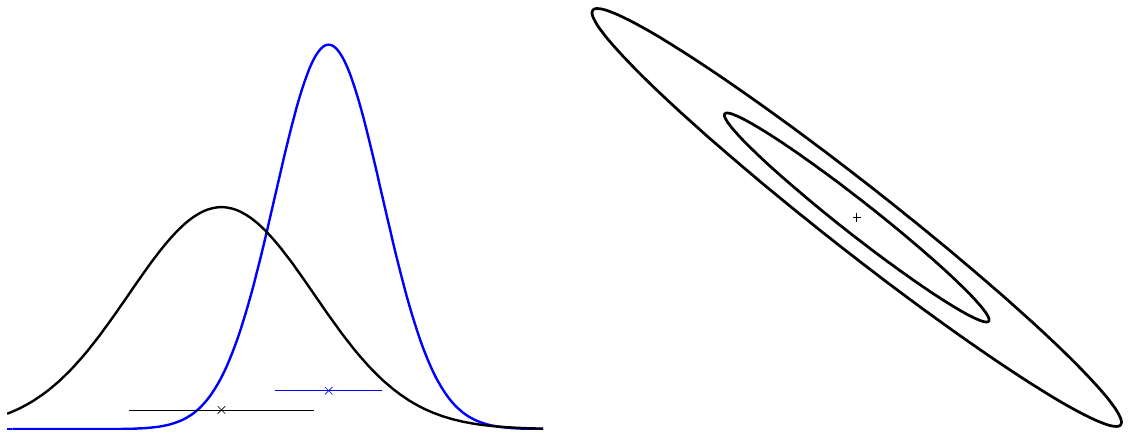
\includegraphics[width=0.9\textwidth]{gaussDist1.png}
    \end{figure}

    \begin{equation*}
      \begin{array}{c}
        p(\bx|\bmu,\bSig) = \gaussN(\bmu,\bSig) = (2\pi)^{-D/2} |\bSig|^{-1/2} \exp \left( - \frac{1}{2} (\bx - \bmu)^T \bSig^{-1} (\bx - \bmu) \right) \\
        \bmu \text{: mean vector, } \bSig \text{: covariance matrix}
      \end{array}
    \end{equation*}
  \end{frame}

  \begin{frame}
    \frametitle{Conditional and Marginal of a Gaussian}

    \begin{figure}
      \centering
      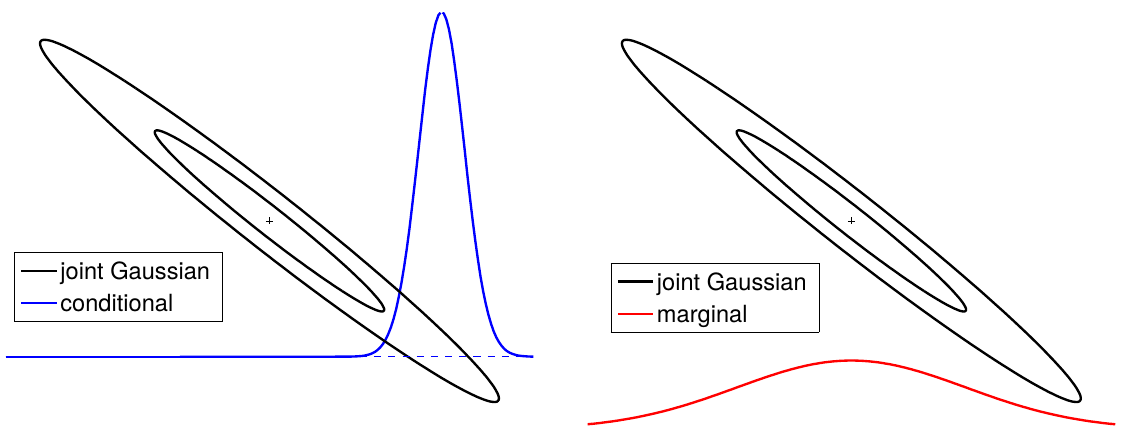
\includegraphics[width=\textwidth]{gaussDist2.png}
    \end{figure}

    \begin{center}
      \textcolor{blue}{Conditional} and \textcolor{red}{Marginal} of a joint Gaussian is also Gaussian.
    \end{center}

  \end{frame}

  \begin{frame}
    \frametitle{What is a Gaussian Process?}
    Generalization of a multivariate Gaussian to \textcolor{red}{infinitely many variables}.

    \begin{block}{}
      \textbf{Definition}: \emph{Gaussian Process is a collection of random variables, any finite collection of which are Gaussian Distributed.}
    \end{block}

    \pause

    Gaussian \textcolor{blue}{distribution}: mean \textcolor{red}{vector}, $\bmu$, and covariance \textcolor{red}{matrix} $\bSig$:
    \begin{equation*}
      \mathbf{f} = (f_1,\dots,f_n)^T \sim \gaussN(\bmu,\bSig),~~\text{indices } i = 1,\dots,n
    \end{equation*}

    \pause

    Gaussian \textcolor{blue}{process}: mean \textcolor{red}{function}, $m(x)$, and covariance \textcolor{red}{function} $k(x,x')$:
    \begin{equation*}
      f(x) \sim \gp(m(x),k(x,x')),~~\text{indices: } x
    \end{equation*}
  \end{frame}

  \begin{frame}
    \frametitle{Marginalization Property}
    How can we represent infinite mean vector and infinite covariance matrix? \\~

    ...luckily saved by \emph{marginalization property}:

    \begin{equation*}
      p(\bx) = \int p(\bx,\by)d \by
    \end{equation*}

    \pause

    For Gaussians:

    \begin{equation*}
      \begin{array}{c}
        p(\bx, \by) = \gaussN \left(\begin{bmatrix} \ba \\ \bb \end{bmatrix}, \begin{bmatrix} \bA & \bB \\ \bB^T & \bC \end{bmatrix} \right) \\~\\
        p(\bx) = \gaussN(\ba,\bA)
      \end{array}
    \end{equation*}
  \end{frame}

  \begin{frame}
    \frametitle{Random sampling from Gaussian Process}
    Considering one dimensional Gaussian process:

    \begin{equation*}
      p(f(x)) \sim \gp \left( m(x) = 0, k(x,x') = \exp \left( - \frac{1}{2} (x - x')^2 \right) \right)
    \end{equation*}

    \pause

    Sampling is done by focusing on subset $\boldf = (f(x_1), f(x_2),\dots,f(x_n))^T$:

    \begin{equation*}
      \boldf \sim \gaussN(0,\bSig) \text{, where } \bSig_{ij} = k(x_i,x_j)
    \end{equation*}

    Coordinates of $\boldf$ are plot as a function of corresponding $x$
  \end{frame}

  \begin{frame}
    \frametitle{Random sample for single dimension}

    \begin{figure}
      \centering
      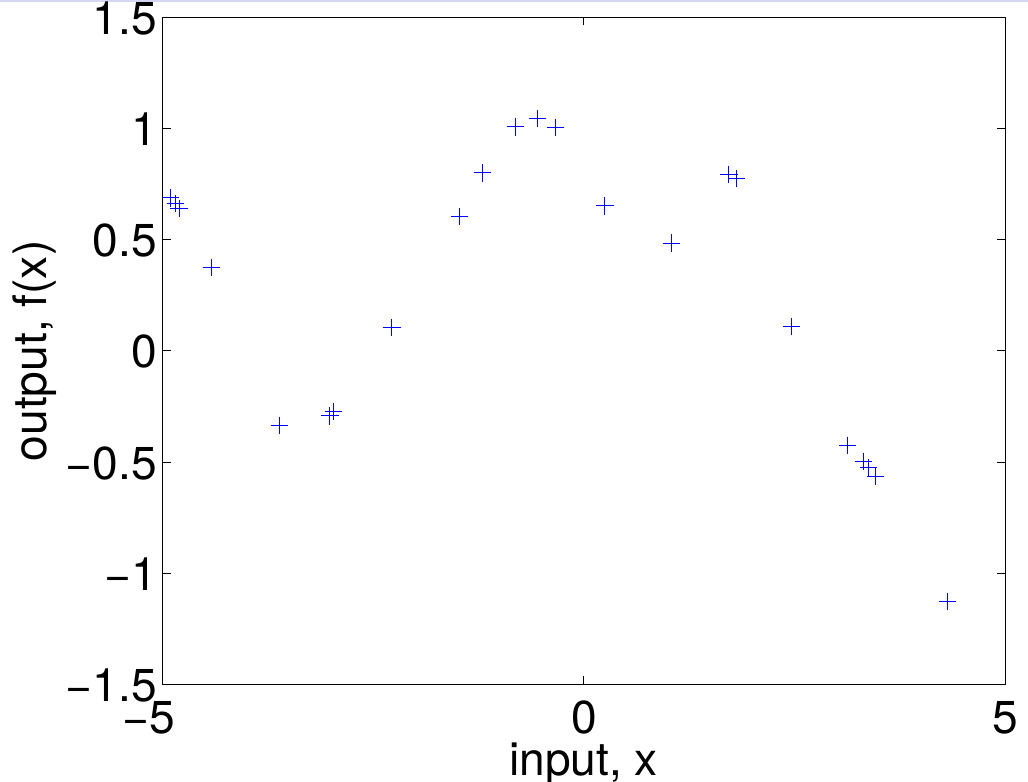
\includegraphics[width=0.8\textwidth]{gpSample.png}
    \end{figure}
  \end{frame}

  \begin{frame}
    \frametitle{2 Dimensional Gaussian Process Sample}

    \begin{figure}
      \centering
      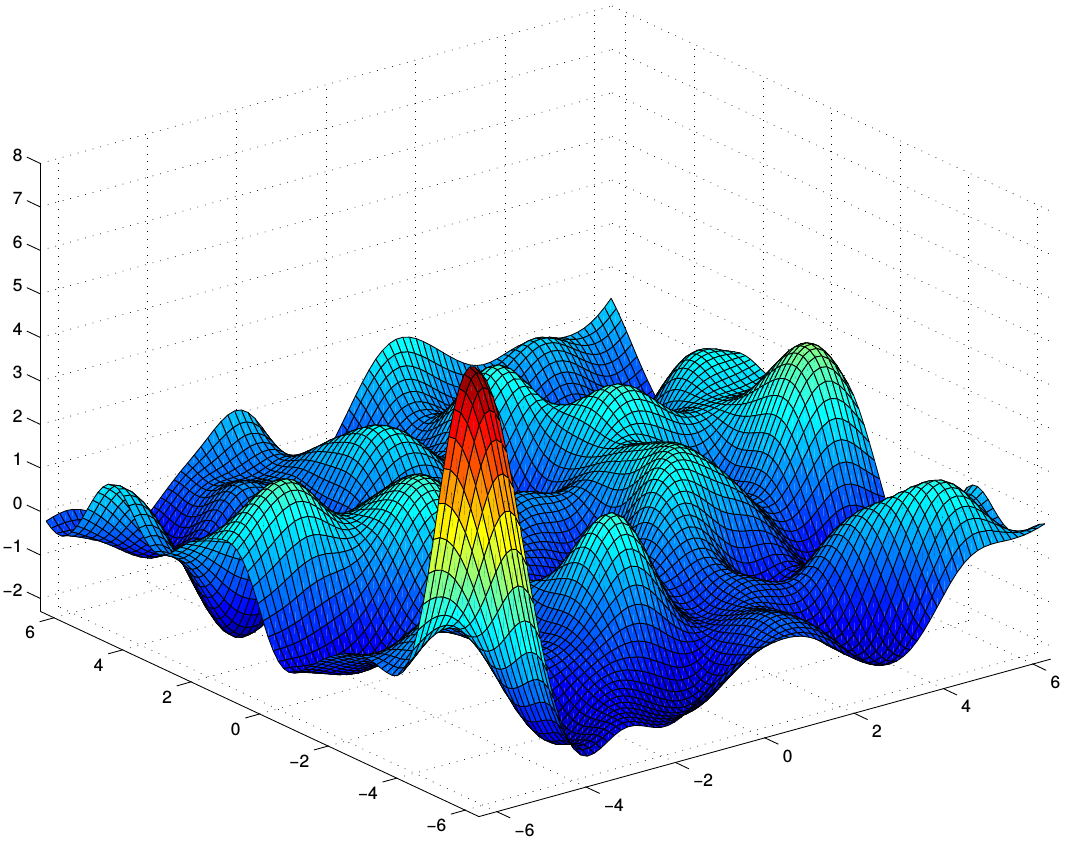
\includegraphics[width=0.8\textwidth]{gpSample2.png}
    \end{figure}
  \end{frame}

  \begin{frame}
    \frametitle{Sequential Generation of Samples}
    Factorize the joint distribution and generate function values sequentially:

    \begin{equation*}
      p(f_1,\dots,f_n|\bx_1,\dots,\bx_n) = \prod_{i=1}^{n} p(f_i|f_{i-1},\dots,f_1,\bx_1,\dots,\bx_n)
    \end{equation*}

    \pause

    What do individual terms look like?

    \begin{equation*}
      \begin{array}{c}
        p(\bx,\by) = \gaussN\left(\begin{bmatrix} \ba \\ \bb \end{bmatrix}, \begin{bmatrix} \bA & \bB \\ \bB^T & \bC \end{bmatrix} \right) \\~\\
        p(\bx|\by) = \gaussN(\ba + \bB \bC^{-1} (\by-\bb), \bA - \bB
         \bC^{-1}\bB^T)
      \end{array}
    \end{equation*}
  \end{frame}

  \section{Inference using Gaussian Processes}

  \begin{frame}
    \frametitle{Parametric Model and Maximum Likelihood}
    Parametric Model:
      \begin{itemize}
        \item data: $\bx, \by$
        \item model: $\by = f_w(\bx) + \epsilon$
      \end{itemize}

    \pause

    Gaussian Likelihood:
      \begin{equation*}
        \textcolor{red}{p(\by|\bx, \bw, M)} \propto \prod_i \exp \left( - \frac{ (y_i - f_{\bw}(x_i))^2}{2 \sigma_{noise}^2} \right)
      \end{equation*}

    \pause

    Maximizing Likelihood:
      \begin{equation*}
        \bw_{ML} = \argmax_{\bw} \textcolor{red}{p(\by|\bx,\bw,M)}
      \end{equation*}

    \pause

    Making predictions:
      \begin{equation*}
        p(y^*|x^*,\bw_{ML},M)
      \end{equation*}
  \end{frame}

  \begin{frame}
    \frametitle{Parametric Model and Bayesian Inference}
    Parametric Model:
      \begin{itemize}
        \item data: $\bx, \by$
        \item model: $\by = f_w(\bx) + \epsilon$
      \end{itemize}

    \pause

    Gaussian Likelihood:
      \begin{equation*}
        \textcolor{red}{p(\by|\bx, \bw, M)} \propto \prod_i \exp \left( - \frac{ (y_i - f_{\bw}(x_i))^2}{2 \sigma_{noise}^2} \right)
      \end{equation*}

    \pause

    Prior over parameters:
      \begin{equation*}
        \textcolor{blue}{p(\bw|M)}
      \end{equation*}

    \pause

    Posterior parameter distribution:
      \begin{equation*}
        \textcolor{green}{p(\bw|\bx,\by,M)} = \frac{\textcolor{blue}{p(\bw|M)} \textcolor{red}{p(\by|\bx, \bw, M)}}{p(\by|\bx,M)}
      \end{equation*}
  \end{frame}

  \begin{frame}
    \frametitle{Parametric Model and Bayesian Inference}

    Making predictions:
      \begin{equation*}
        p(y^*|x^*,\bx,\by,M) = \int p(y^*|\bw,x^*,M) \textcolor{green}{p(\bw|\bx,\by,M)} d\bw
      \end{equation*}

    \pause

    Marginal Likelihood:
      \begin{equation*}
        p(\by|\bx,M) = \int \textcolor{blue}{p(\bw|M)} \textcolor{red}{p(\by|\bx, \bw, M)} d\bw
      \end{equation*}

    \pause

    Model probability:
      \begin{equation*}
        p(M|\bx,\by) = \frac{p(M)p(\by|\bx,M)}{p(\by|\bx)}
      \end{equation*}

    \pause

    \begin{center}
      \textbf{Problem: integrals are intractable for most interesting models!}
    \end{center}
  \end{frame}

  \begin{frame}
    \frametitle{Non-parametric Gaussian Process Models}
    Parameters are replaced by ``function'' itself!

    \pause

    Gaussian Likelihood:
      \begin{equation*}
        \textcolor{red}{\by|\bx,f(x),M} \sim \gaussN(\boldf, \sigma^2_{noise}I)
      \end{equation*}

    \pause

    Gaussian Process Prior:
      \begin{equation*}
        \textcolor{blue}{f(x)|M} \sim \gp(m(x) = 0, k(x,x'))
      \end{equation*}

    \pause

    Leading to Gaussian Process Posterior:
      \begin{equation*}
        \begin{array}{c}
          \textcolor{green}{f(x)|\bx,\by,M} \sim \gp ( m_{\text{post}}(x) = k(x,\bx)[K(\bx,\bx) + \sigma^2_{noise}I]^{-1} \by, \\[0.2cm]
          \; k_{\text{post}}(x,x') =  k(x,x') - k(x,\bx)[K(\bx,\bx) + \sigma^2_{noise}I]^{-1} k(\bx,x') )
        \end{array}
      \end{equation*}
    \end{frame}

  \begin{frame}
    \frametitle{Prior and Posterior for $\gp$ Learning}

    \begin{figure}
      \centering
      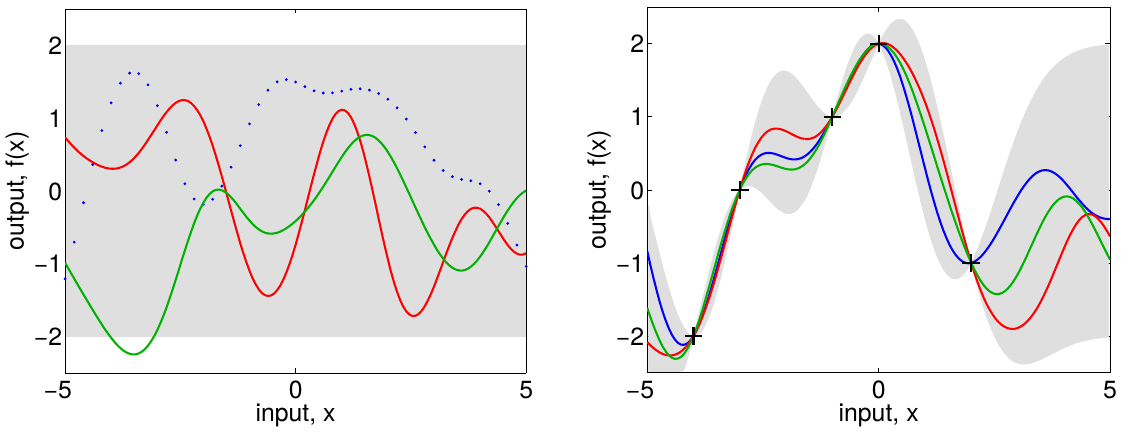
\includegraphics[width=\textwidth]{gpRegression.png}
    \end{figure}

    Gaussian Process Predictive Distribution:
      \begin{equation*}
        \begin{array}{c}
          p(y^*|x^*,\bx,\by) \sim \gaussN ( k(x^*,\bx)[K + \sigma^2_{noise}]^{-1}\by, \\[0.2cm]
          \; k(x*,x*) - k(x^*,\bx)[K + \sigma^2_{noise}I]^{-1} k(\bx,x^*) )
        \end{array}
      \end{equation*}

  \end{frame}

  \begin{frame}
    \frametitle{Graphical Model for Gaussian Processes}

    \begin{columns}
      \begin{column}{0.55\textwidth}
        \begin{figure}
          \centering
          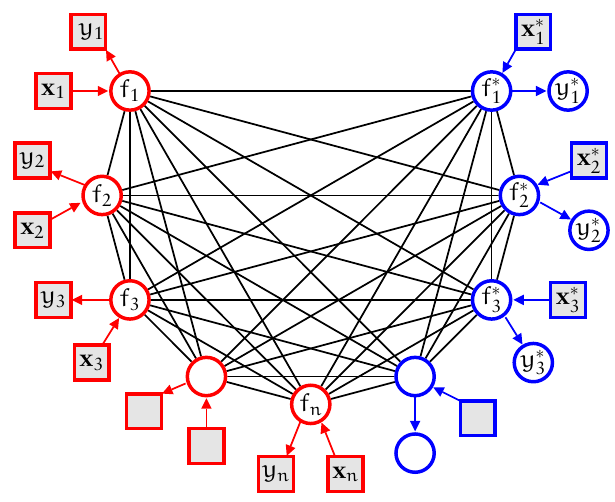
\includegraphics[width=\textwidth]{gpModel.png}
        \end{figure}
      \end{column}
      \begin{column}{0.45\textwidth}
        \begin{itemize}
          \item All pairs of latent variables are connected.\\~
          \item Predictions $y^*$ depend only on corresponding latent $f^*$.\\~
          \item Adding $x_m^*,y_m^*,f_m^*$ does not influence the distribution. Guaranteed by marginalization property.\\~
        \end{itemize}
      \end{column}
    \end{columns}

    \begin{center}
      \textbf{Explains why inference uses finite amount of computation!}
    \end{center}
  \end{frame}

  \begin{frame}
    \frametitle{Interpretation of $\gp$ Inference}
    Recalling predictive distribution:

    \begin{equation*}
      \begin{array}{c}
        p(y^*|x^*,\bx,\by) \sim \gaussN ( k(x^*,\bx)[K + \sigma^2_{noise}]^{-1}\by, \\[0.2cm]
        \; k(x*,x*) - k(x^*,\bx)[K + \sigma^2_{noise}I]^{-1} k(\bx,x^*) )
      \end{array}
    \end{equation*}

    \pause

    Mean can be linearly represented as:

    \begin{equation*}
      \bmu(x^*) = k(x^*,\bx)[K + \sigma_{noise}^2]^{-1} \by = \sum_{i=1}^n \beta_iy_i = \sum_{i=1}^n \alpha_ik(x^*,x_i)
    \end{equation*}

    \pause

    Variance is composed of two terms:

    \begin{equation*}
      \bSig{x^*} = \underset{\text{\textbf{prior variance}}}{k(x*,x*)} - \underset{\text{\textbf{variance by data}}}{k(x^*,\bx)[K + \sigma^2_{noise}I]^{-1} k(\bx,x^*)}
    \end{equation*}

    \textbf{Note that the variance is independent of observed outputs $\by$}.
  \end{frame}

  \begin{frame}
    \frametitle{Optimizing Marginal Likelihood}
    \begin{equation*}
      \log p(\by|\bx,M) = - \textcolor{blue}{\frac{1}{2} \by^T K^{-1} \by} - \textcolor{red}{\frac{1}{2} \log|K|} - \frac{n}{2} \log (2\pi)
    \end{equation*}

    is a combination of \textcolor{blue}{data fit} and \textcolor{red}{complexity penalty} terms. Occam's razor is automatic!\\~\\

    \pause

    \textcolor{blue}{Learning} in Gaussian process models involves finding:
      \begin{itemize}
        \item Form of covariance matrix
        \item Unknown hyperparameter values $\theta$
      \end{itemize}

    \pause

    ~\\ This can be done by optimizing the marginal likielihood:

    \begin{equation*}
      \frac{\partial \log p(\by|\bx,\theta,M)}{\partial \theta_j} = \frac{1}{2} \by^T K^{-1} \frac{\partial K}{\partial \theta_j} K^{-1} \by - \frac{1}{2} \text{trace} \left( K^{-1} \frac{\partial K}{\partial \theta_j} \right)
    \end{equation*}
  \end{frame}

  \begin{frame}
    \frametitle{Example: Length Parameter Learning}

    Covariance function: $k(x,x') = \nu^2 \exp \left( - \frac{(x - x')^2}{2l^2} \right) + \sigma_{noise}^2 \delta_{xx'}$

    \begin{figure}
      \centering
      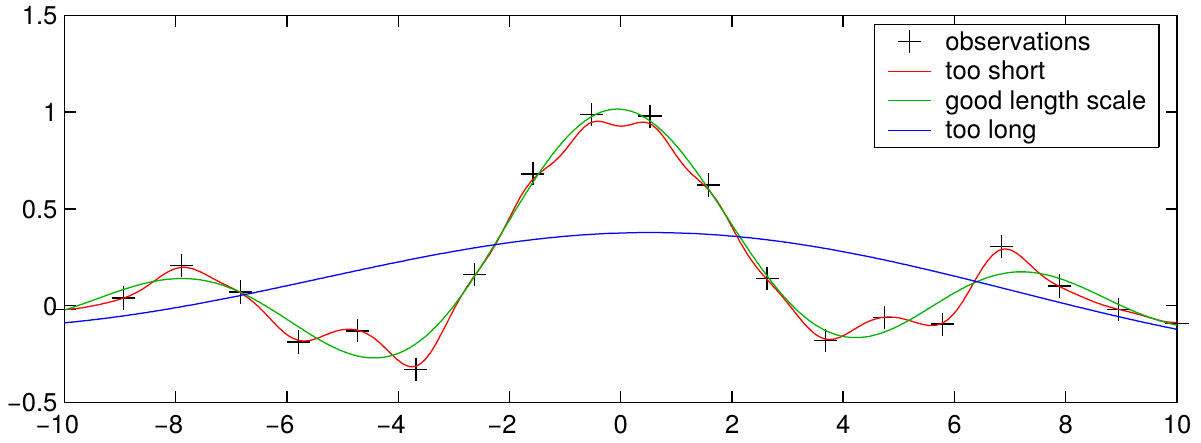
\includegraphics[width=0.8\textwidth]{gpLearning.png}
    \end{figure}

    Posterior mean function is plotted for 3 different length scales, green curve maximizes marginal likelihood. \textcolor{blue}{Although exact fit for data can be found, marginal likelihood does not favour this!}
  \end{frame}

  \begin{frame}
    \frametitle{Why does Bayesian Inference work?: Occam's Razor}

    \begin{figure}
      \centering
      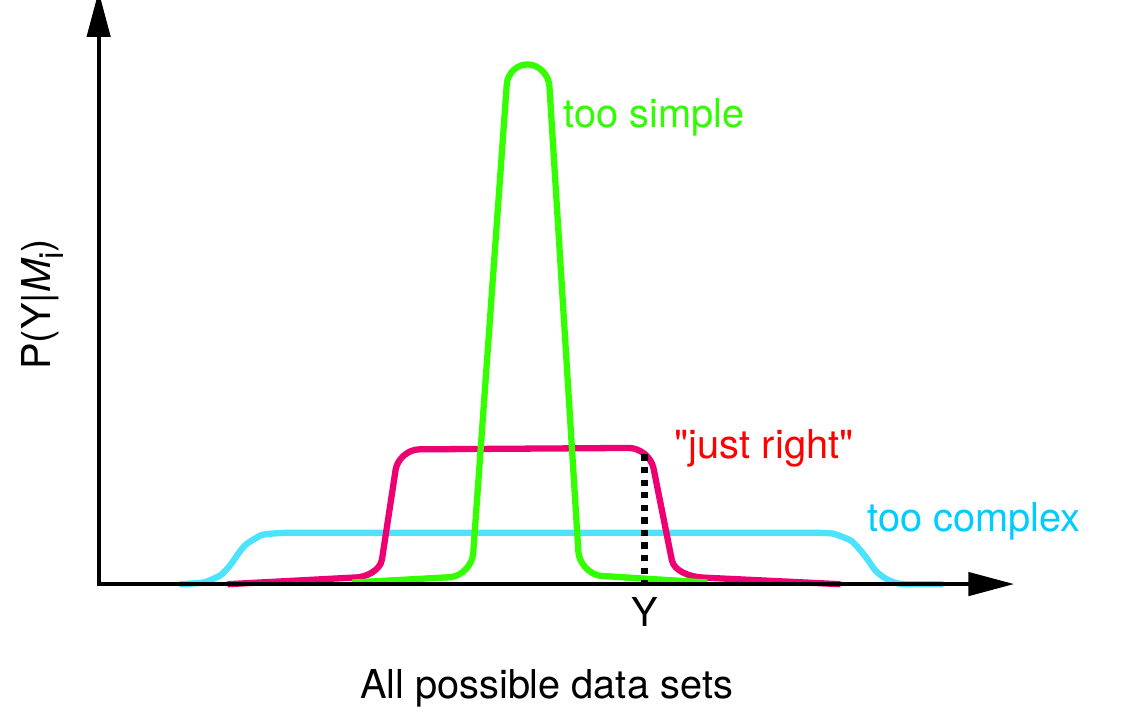
\includegraphics[width=0.9\textwidth]{occamsRazor.png}
    \end{figure}
  \end{frame}

  \begin{frame}
    \frametitle{Analogous Example}

    Task: Fitting variance, $\sigma^2$, of zero-mean Gaussian to $n$ scalar observations.

    \begin{figure}
      \centering
      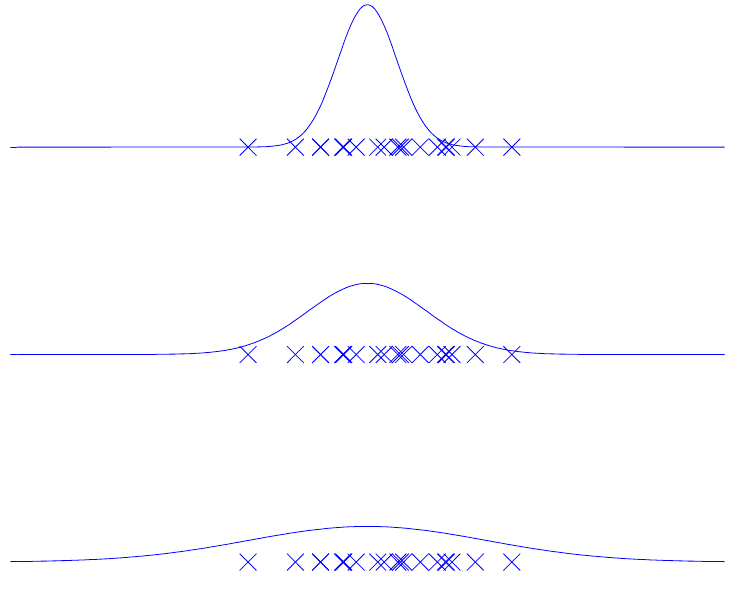
\includegraphics[height=0.6\textheight]{occamsRazor2.png}
    \end{figure}

    Log likelihood is $\log p(y|\mu,\sigma^2) = \textcolor{blue}{- \frac{1}{2} \sum \frac{(y_i - \mu)}{\sigma^2}} \textcolor{red}{- \frac{n}{2} \log(\sigma^2)} - \frac{n}{2} \log(2\pi)$
  \end{frame}

  \section{Covariance Functions}

  \begin{frame}
    \frametitle{Covariance Function for Linear Models}
    Consider the class of linear functions:

    \begin{equation*}
      f(x) = ax + b,~\text{where } a \sim \gaussN(0,\alpha), \text{ and } b \sim \gaussN(0,\beta)
    \end{equation*}

    \pause

    We can compute the mean as:

    \begin{equation*}
      \mu(x) = E[f(x)] = \int \int f(x) p(a) p(b) da db = \int a x p(a) da + \int b p(b) db = 0
    \end{equation*}

    \pause

    and covariance function as:

    \begin{equation*}
      \begin{array}{c}
        k(x,x') = E[(f(x) - 0)(f(x') - 0)] = \int \int (ax+b)(ax'+b)p(a)p(b)dadb\\[0.2cm]
        = \int a^2 x x' p(a) da + \int b^2 p(b) db + (x + x') \int a b p(a) p(b) da db = \alpha x x' + \beta
      \end{array}
    \end{equation*}
  \end{frame}

  \begin{frame}
    \frametitle{Regression with Basis Functions}
    Consider the class of linear functions:

    \begin{equation*}
      \begin{array}{cc}
        f(x) & = \lim_{n \leftarrow \infty} \frac{1}{n} \sum_i \gamma_i \exp(-(x - i/n)^2),~\text{where } \gamma_i \sim \gaussN(0,1), \forall i \\[0.2cm]
        & = \int_{- \infty}^{\infty} \gamma(u) \exp(-(x - u)^2)du,~\text{where}~\gamma(u) \sim \gaussN(0,1), \forall u
      \end{array}
    \end{equation*}

    \pause

    Mean function is:

    \begin{equation*}
      \mu(x) = E[f(x)] = \int_{- \infty}^{\infty} \exp(-(x-u)^2) \int_{- \infty}^{\infty} \gamma p(\gamma) d\gamma du = 0
    \end{equation*}
  \end{frame}

  \begin{frame}
    \frametitle{Regression with Basis Functions}

    Covariance function is:

    \begin{equation*}
      \begin{array}{c}
        E[f(x)f(x')] = \int \exp ( - (x-u)^2 - (x' - u)^2)du \\[0.2cm]
        = \int \exp \left( -2 \left( u - \frac{x + x'}{2} \right)^2 + \frac{(x- x')^2}{2} - x^2 -x'^2 \right) du \\[0.2cm]
        \propto \exp \left( - \frac{(x - x')^2}{2} \right)
      \end{array}
    \end{equation*}

    \pause

    \begin{center}
      \textbf{Using squared exponential covariance function is equivalent to regression using infinitely many bell-shaped basis functions!}
    \end{center}
  \end{frame}

  \begin{frame}
    \frametitle{Using finite basis functions can be dangerous!}

    \begin{figure}
      \centering
      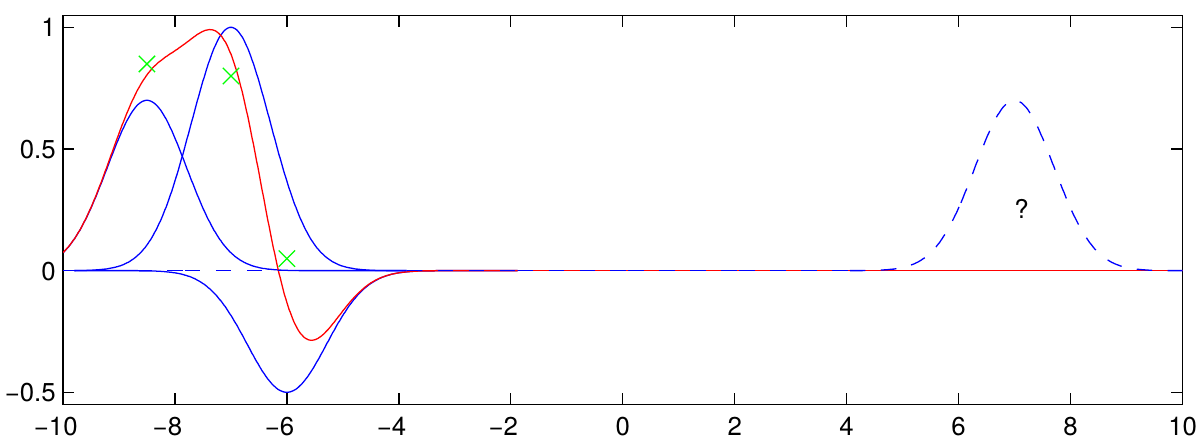
\includegraphics[width=\textwidth]{finiteBasis.png}
    \end{figure}
  \end{frame}

  \begin{frame}
    \frametitle{Model Selection in Practice}

    Two types of selection: \emph{form} and \emph{parameters} of covariance function.\\~

    \textcolor{blue}{Hyperparameters} form a herarchical model. Eg, ARD Covariance Function:

    \begin{equation*}
      k(x,x') = \nu_0^2 \exp \left( - \sum_{d=1}^D \frac{(x_d - x_d')^2}{2\nu_d^2} \right),~\text{hyperparameters}~\theta = (\nu_0,\dots,\sigma_{noise}^2)
    \end{equation*}

    \begin{figure}
      \centering
      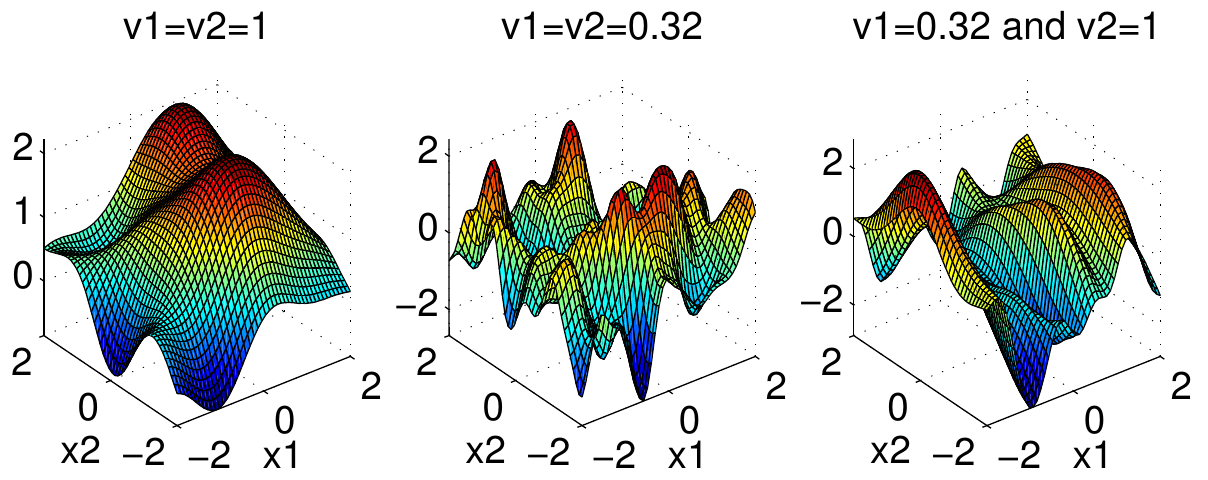
\includegraphics[width=0.8\textwidth]{hyperparameters.png}
    \end{figure}
  \end{frame}

  \begin{frame}
    \frametitle{Rational Quadratic (RQ) Covariance Function}

    \begin{equation*}
      k_{RQ}(r) = \left( 1 + \frac{r^2}{2 \alpha l^2} \right)^{- \alpha}
    \end{equation*}

    with $\alpha, l > 0$ can be seen as an infinite sum of squared exponential (SE) covariance functions with differen length-scales.\\~

    \pause

    Using $\tau = l^2$ and $p(\tau | \alpha, \beta) \propto \tau^{\alpha - 1} \exp (- \alpha \tau / \beta)$:

    \begin{equation*}
      \begin{array}{c}
        k_{RQ}(r) = \int p(\tau | \alpha, \beta) k_{SE}(r| \tau) d\tau \\
        \propto \int \tau^{\alpha - 1} \exp \left( - \frac{\alpha \tau}{\beta} \right) \exp \left( - \frac{\tau r^2}{2} \right) d \tau \propto \left( 1 + \frac{r^2}{2 \alpha l^2} \right)^{- \alpha}
      \end{array}
    \end{equation*}
  \end{frame}

  \begin{frame}
    \frametitle{Rational Quadratic Covariance Function}

    \begin{figure}
      \centering
      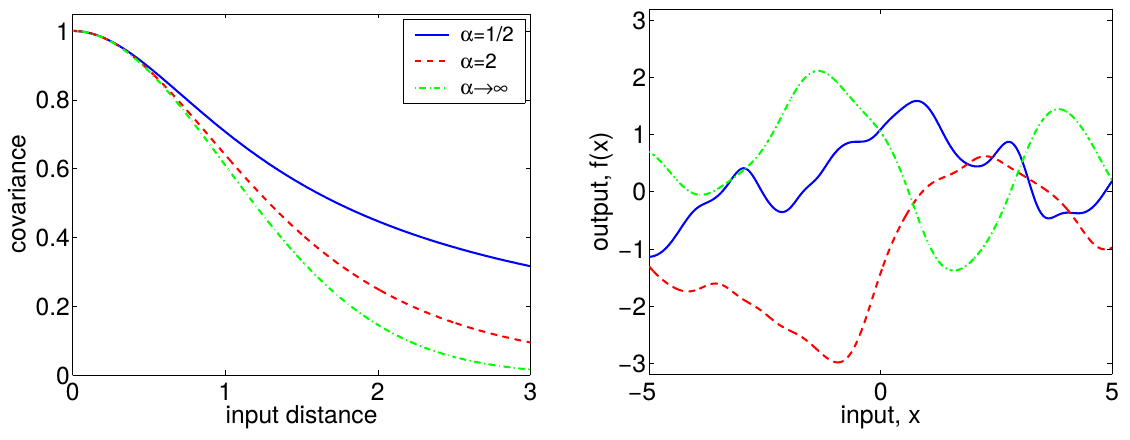
\includegraphics[width=0.9\textwidth]{rationalCovFunc.png}
    \end{figure}

    \begin{center}
      Limit $\alpha \leftarrow \infty$ of the RQ covariance function is SE.
    \end{center}
  \end{frame}

  \begin{frame}
    \frametitle{Matern Covariance Function}

    \begin{equation*}
      k(x,x') = \frac{1}{\Gamma(\nu) 2^{\nu - 1}} \left[ \frac{\sqrt{2 \nu}}{l} |x - x'| \right]^{\nu} K_{\nu} \left( \frac{\sqrt{2 \nu}{l}} |x - x'| \right)
    \end{equation*}

    where $K_{\nu}$ is a Bessel function of order $\nu$, and $l$ is the length scale.\\~

    \pause

    Samples of Matern forms are $\lfloor \nu - 1 \rfloor$ times differentiable.

    \begin{itemize}
      \item $k_{\nu = 5/2} (r) = \left( 1 + \frac{\sqrt{5}r}{l} + \frac{5 r^2}{3 l^2} \right) \exp \left( - \frac{\sqrt{5}r}{l} \right)$: Twice differentiable
      \item $k_{\nu \leftarrow \infty} (r) = \exp \left( - \frac{r^2}{2 l^2} \right)$: Smooth (Infinite differentiable)
    \end{itemize}
  \end{frame}

  \begin{frame}
    \frametitle{Matern Covariance Function}
    Univariate Matern covariance functions with unit length scale and unit variance:

    \begin{figure}
      \centering
      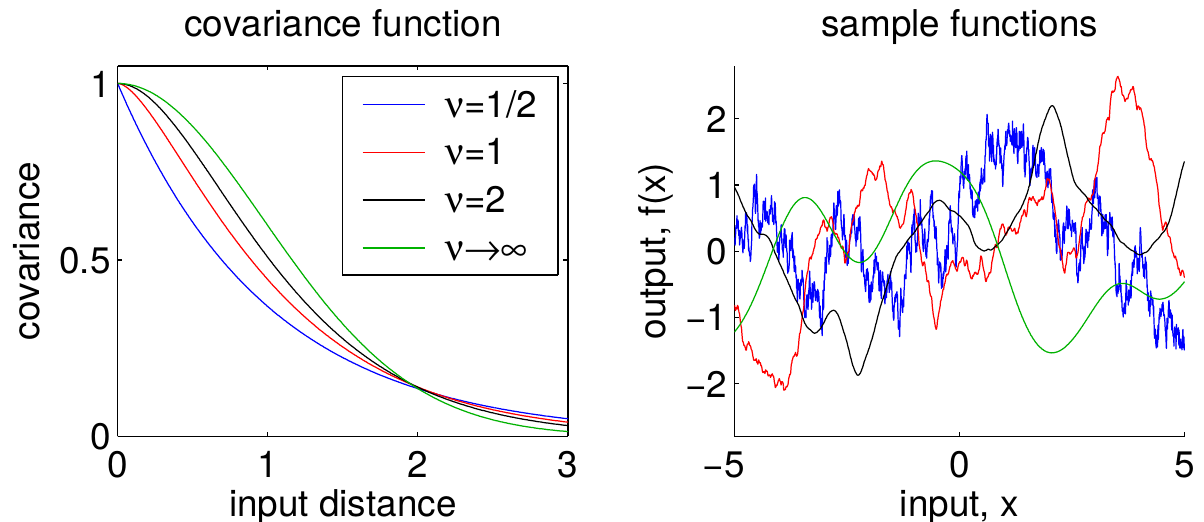
\includegraphics[width=0.9\textwidth]{maternCovFunc.png}
    \end{figure}
  \end{frame}

  \begin{frame}
    \frametitle{Periodic Covariance Function}
    Periodic covariance functions can be obtained by mapping $x$ to $u = (\sin(x), \cos(x))^T$ and combine with SE covariance function:

    \begin{equation*}
      k_{periodic} (x,x') = \exp \left( - \frac{2 \sin^2(\pi (x - x'))}{l^2} \right)
    \end{equation*}

    \begin{figure}
      \centering
      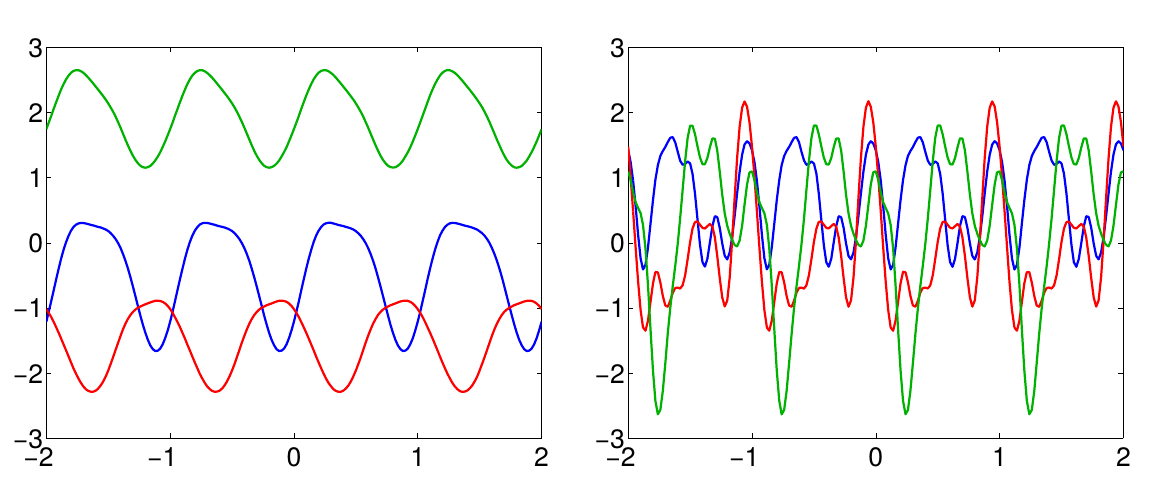
\includegraphics[width=0.8\textwidth]{periodicCovFunc.png}
      \caption*{3 random samples with: left $l > 1$ and right $l < 1$}
    \end{figure}
  \end{frame}

  \section{Application to CO$_2$ Prediction Problem}

  \begin{frame}
    \frametitle{Prediction Problem}

    \begin{figure}
      \centering
      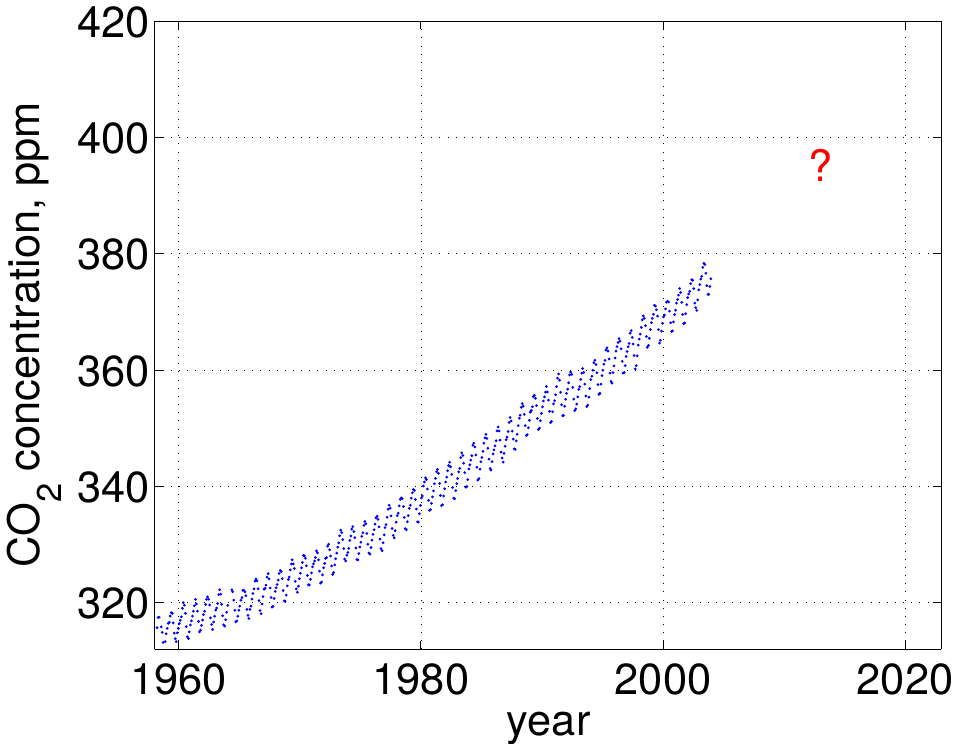
\includegraphics[width=0.8\textwidth]{prediction1.png}
    \end{figure}
  \end{frame}

  \begin{frame}
    \frametitle{Covariance Functions}

    \begin{itemize}
      \item long term smooth trend (\textcolor{blue}{squared exponential})
        \begin{equation*}
          k_1(x,x') = \theta_1^2 \exp \left( \frac{(x - x')^2}{\theta_2^2} \right)
        \end{equation*}
      \item seasonal trend (\textcolor{blue}{quasi-periodic smooth})
        \begin{equation*}
          k_2(x,x') = \theta_3^2 \exp \left( - \frac{2 \sin^2 (\pi (x - x'))}{\theta_5^2} \right) \times \exp \left( \frac{(x - x')^2}{2 \theta_4^2} \right)
        \end{equation*}
      \item short and medium term anomaly (\textcolor{blue}{rational quadratic})
        \begin{equation*}
          k_3(x,x') = \theta_6^2 \left( 1 + \frac{(x - x')^2}{2 \theta_8 \theta_7^2} \right)^{- \theta_8}
        \end{equation*}
    \end{itemize}

    \begin{equation*}
      k(x,x') = k_1(x,x') + k_2(x,x') + k_3(x,x') + \text{noise kernel}
    \end{equation*}
  \end{frame}

  \begin{frame}
    \frametitle{Carbon Dioxide Predictions}

    \begin{figure}
      \centering
      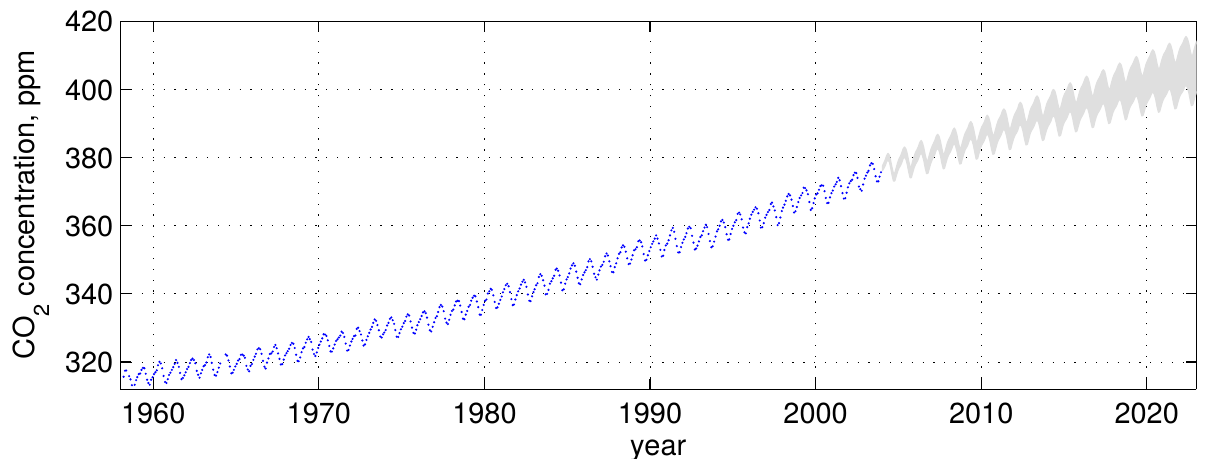
\includegraphics[width=\textwidth]{prediction2.png}
    \end{figure}
  \end{frame}

  \begin{frame}
    \frametitle{Long and Medium-term Predictions}

    \begin{figure}
      \centering
      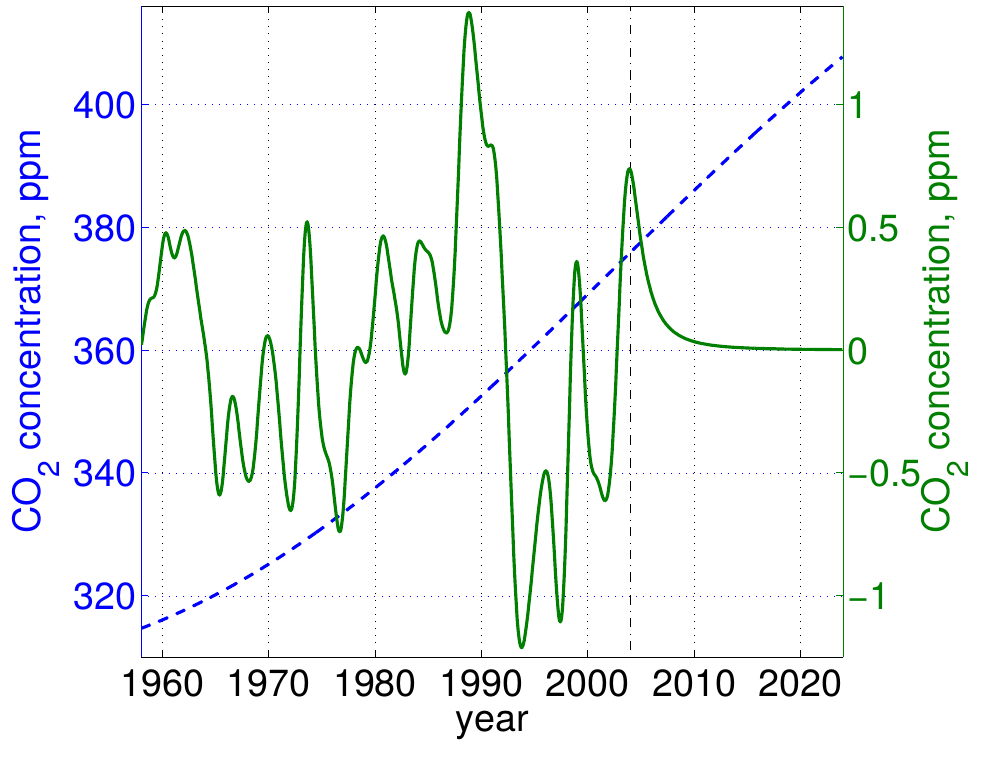
\includegraphics[width=0.8\textwidth]{prediction3.png}
    \end{figure}
  \end{frame}

  \begin{frame}
    \frametitle{Mean Seasonal Component}

    \begin{figure}
      \centering
      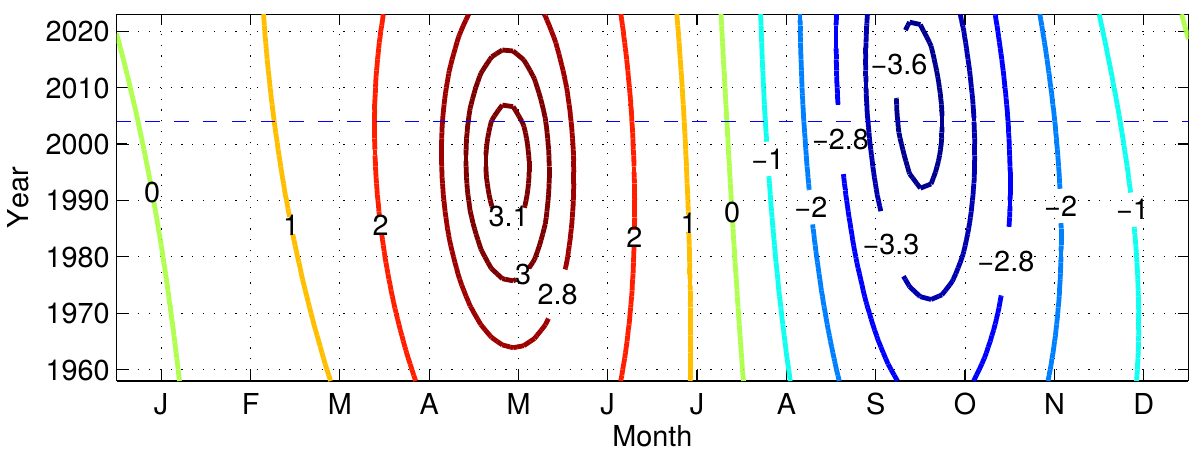
\includegraphics[width=\textwidth]{prediction4.png}
    \end{figure}
  \end{frame}

  \section{Conclusions}

  \begin{frame}
    \frametitle{Conclusions}

    \textbf{Complex non-linear inference problems can be solved by manipulating plain old Gaussian Distributions}

    \begin{itemize}
      \item Bayesian inference is tractable for GP Regression
      \item Predictions are probabilistic
      \item Comparison of different models possible via Marginal Likelihood
    \end{itemize}

    \pause

    \textbf{Scope for research:}

    \begin{itemize}
      \item Interesting covariance functions
      \item Search for efficient approximations and sparse methods
      \item Application to high-dimensional data (Deep Learning)
    \end{itemize}

  \end{frame}
\end{document}
